\chapter{Experiments}
\label{sec:experiments}
The goal of the experiments is to determine the average actual stretch of
estimates $\bar{s}$, and also I find it interesting how the actual stretches
are spread in the stretch interval $[1:3]$ on the two different domains of
graphs I have used in my experiments.

The test data consist of five graphs in two domains. Three road networks and
two internet topologies. All graphs are undirected and all edge weights are
$1$. The graphs are from Stanford Large Network Dataset collection\cite{snapnets} and is
described below.
\begin{description}
  \item[Internet topologies] \hfill
        \begin{description}
        \item[Skitter] \hfill \\
                Created from traceroutes run daily in 2005 - From several
                scattered sources to million destinations. 1696415 nodes,
                11095298 edges. Longest shortest path is 25.
        \item[AS-733] \hfill \\
                A communication network of who-talks-to-whom, constructed from
                BGP (Border Gateway Protocol) logs. 6474 nodes, 13895
                edges. Longest shortest path is 9.
        \end{description}
  \item[Road networks] \hfill
        \begin{description}
        \item[California] \hfill \\
                Road network of California. Intersections and endpoints
                are represented by nodes and the roads connecting these
                intersections or road endpoints are represented by undirected
                edges. 1965206 nodes, 2766607 edges. Longest shortest path is
                849.

        \item[Texas] \hfill \\
                Road network of Texas. Intersections and endpoints
                are represented by nodes and the roads connecting these
                intersections or road endpoints are represented by undirected
                edges. 1379917 nodes and 1921660 edges. Longest shortest path
                is 1054.

        \item[Pennsylvania] \hfill \\
                Road network of Pennsylvania. Intersections and endpoints are
                represented by nodes and the roads connecting these
                intersections or road endpoints are represented by undirected
                edges. 1088092 nodes, 1541898 edges. Longest shortest path is
                786.
        \end{description}

\end{description}

I approached the experiments by generating three approximate distance oracle
data structures per graph, and for each of these data structure sample $1000$
vertex pairs, for which the actual stretch has been computed. For each run
the sampled vertex pairs, used to calculate the actual stretch, are the same.
This has been achieved by seeding the random generator with the same seed when
generating the samples. The idea of using the same samples on the three data
structures for a graph, is that only the random selection of $i$-centers in
\proc{prepro} will then effect fluctuation in the actual stretch observed,
thus some noise is removed.

The results are shown by using plots and tables. The plots I use has stretch
on the $y$-axis, and the $x$-axis shows the percentage of observations with a
stretch equal or less to the corresponding value on the $y$-axis.
I find this plot to give a good intuition about the distribution of the
actual stretch values, and at the same time it is easy to read median and
quantiles from the plot. The plot use a different color for results based
on each of the three data structures. The median, mean and max is calculated
on the unified observations for each graph, thus all 3000 observations per
graph are used to calculate these numbers.

All experiments is conducted on a Macbook Pro with 2.3 GHz (i7-4850HQ)
quad-core Intel Core i7 Haswell processor and 16 GB memory. 
Even with all optimizations described in \autoref{sec:implementation}, the
construction of a data structure takes $\sim75$ minutes for the largest of the
graphs in my experiment and consumes $\sim40$ GB storage. But these numbers are
reasonable.

\section{Road networks}
The plot showing the results for the experiment on the Californian road
network is found in \autoref{fig:ca}, and I find that the large majority of
observations has an actual stretch of $1.1$ or below. The median is $1.05$, the
maximum actual stretch observed is $2.41$ and the mean is $1.08$.
\begin{figure}[htbp]
    \centering
    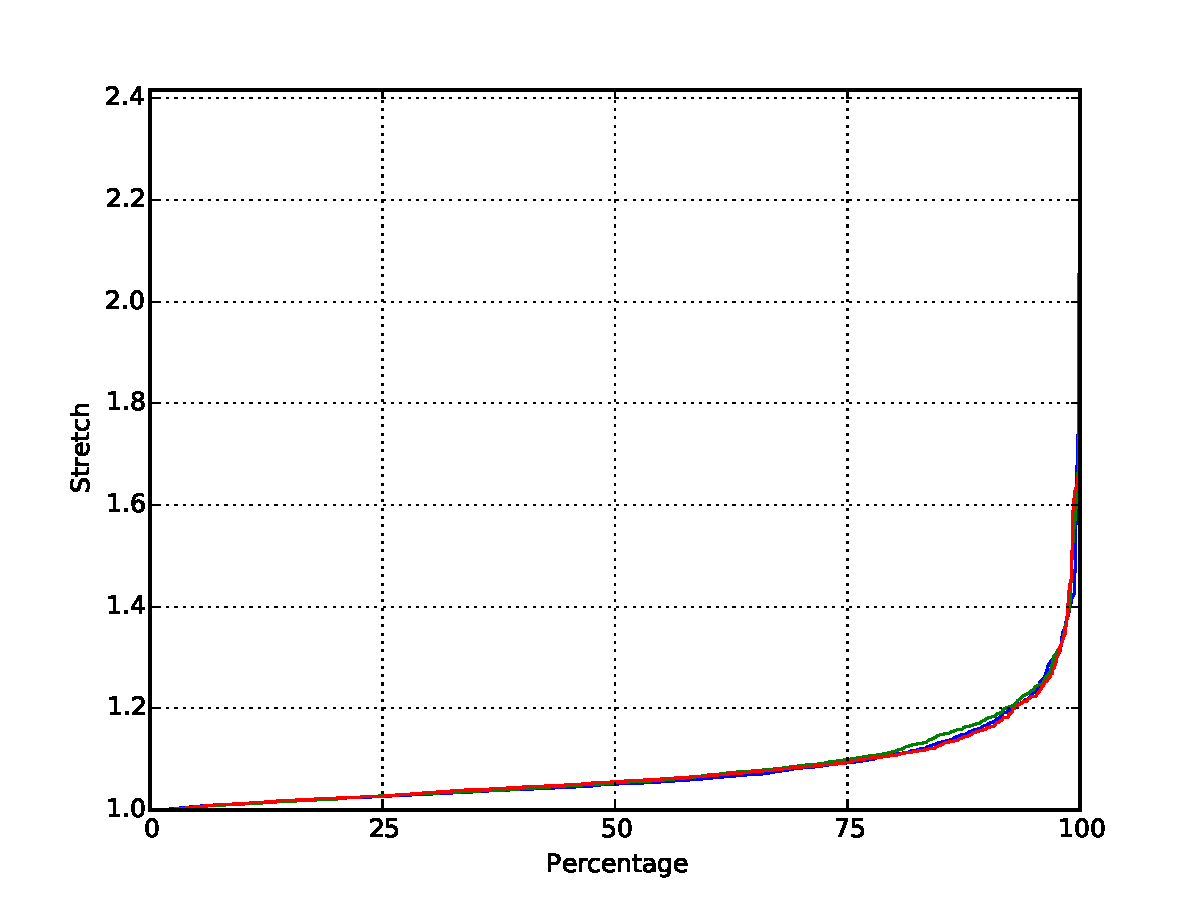
\includegraphics[width=0.8\textwidth]{plots/roadnet_ca.pdf}
    \caption{Actual stretches for California road network, the observations
    from each of the three data structures, has been given different colors.}
    \label{fig:ca}
\end{figure}

For Texas road network the results are very similar. \autoref{fig:tx}
shows how the distribution of the observed actual stretches is more or less
identical to the results found from the graph of California. The experiment
on the road network of Texas shows a median of $1.04$, a mean of $1.06$ and a
maximum actual stretch $2.24$.
\begin{figure}[htbp]
    \centering
    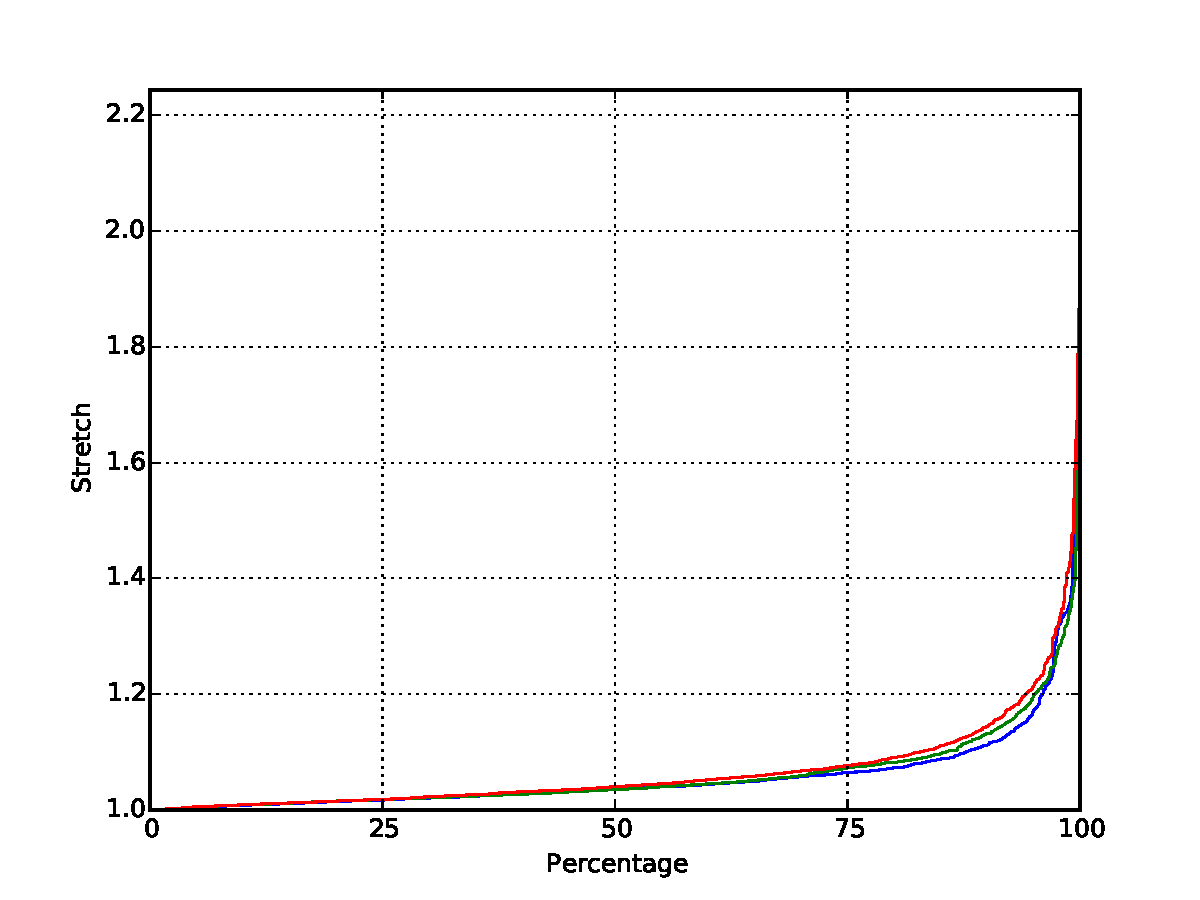
\includegraphics[width=0.8\textwidth]{plots/roadnet_tx.pdf}
    \caption{Actual stretches for Texas road network, the observations
    from each of the three data structures, has been given different colors.}
    \label{fig:tx}
\end{figure}

The graph of Pennsylvania roads, resembles the results from the other road
networks and the experiment returns a median of $1.04$, a mean of $1.07$ and
a maximum observation of $2.33$. \autoref{fig:pa} plots the observations and
it is clear that the shape of the curve and values read from the plot shares
characteristic with the other road networks.

\begin{figure}[htbp]
    \centering
    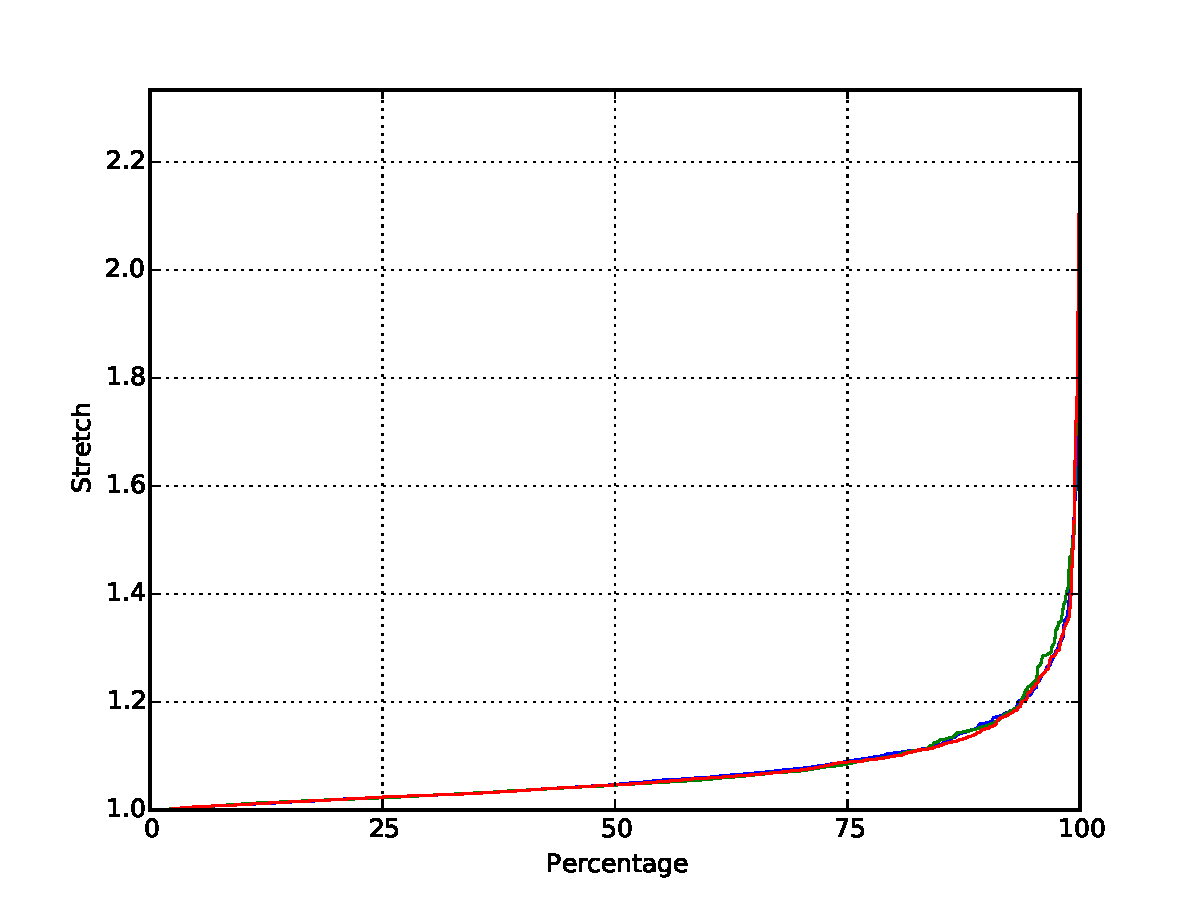
\includegraphics[width=0.8\textwidth]{plots/roadnet_pa.pdf}
    \caption{Actual stretches for Pennsylvania road network, the observations
    from each of the three data structures, has been given different colors.}
    \label{fig:pa}
\end{figure}

The results from running the experiment over the three road network data sets,
indicate that the actual stretches and actual stretch distribution in this
graph domain is very similar and I find the low stretch and low deviations very
impressive. \autoref{tab:roadmap} sums up the results for median, mean, and max.
\begin{table}[htbp]
    \centering
    \begin{tabular}{ l | c | c | c }
        \toprule
             & CA & TX & PA \\
        \midrule
        Median & 1.05 & 1.04 & 1.04 \\
        Max. & 2.41 & 2.24 & 2.33 \\
        \midrule
        Mean. & 1.08 & 1.06 & 1.07 \\
    \end{tabular}
    \caption{Median, maximum and mean for road networks}
    \label{tab:roadmap}
\end{table}
\clearpage

\section{Internet topologies}

For the Skitter topology I find a median of $1.40$ which is substantially
higher than medians found in the road networks. The mean follows the
median and is found to be $1.40$. The maximum actual stretch observed is
$3.0$, which is equal to worst-case. A plot for the experiment is found in
\autoref{fig:skitter}.
\begin{figure}[htbp]
    \centering
    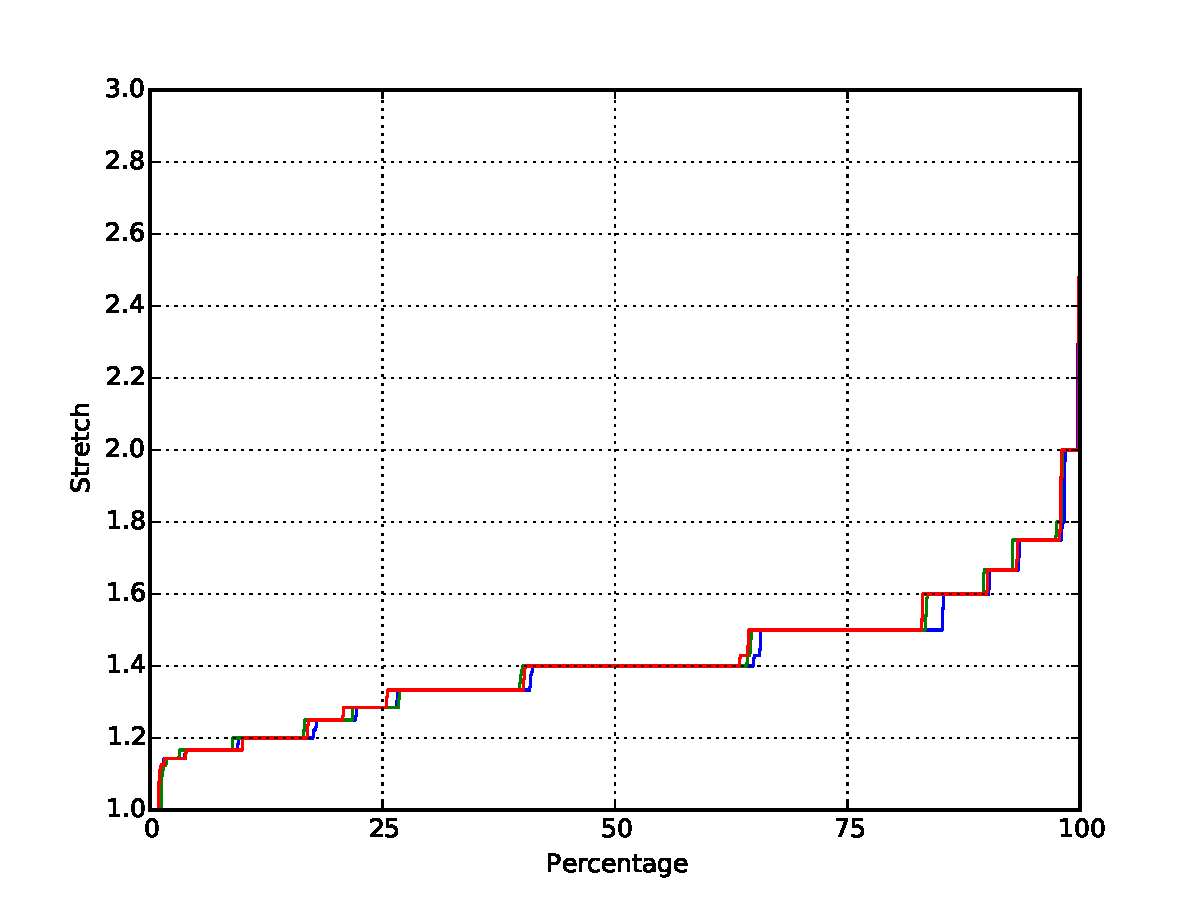
\includegraphics[width=0.8\textwidth]{plots/as_skitter.pdf}
    \caption{Actual stretches for Skitter internet topology, the observations
    from each of the three data structures, has been given different colors.}
    \label{fig:skitter}
\end{figure}

For AS-733 the median is even higher with a value of $1.50$. Also the mean
is higher than we have seen in the other experiments. The mean is $1.56$ and
the maximum actual stretch is again $3.0$. The plot for the stretches of
AS-733 is shown in \autoref{fig:as733}.
\begin{figure}[htbp]
    \centering
    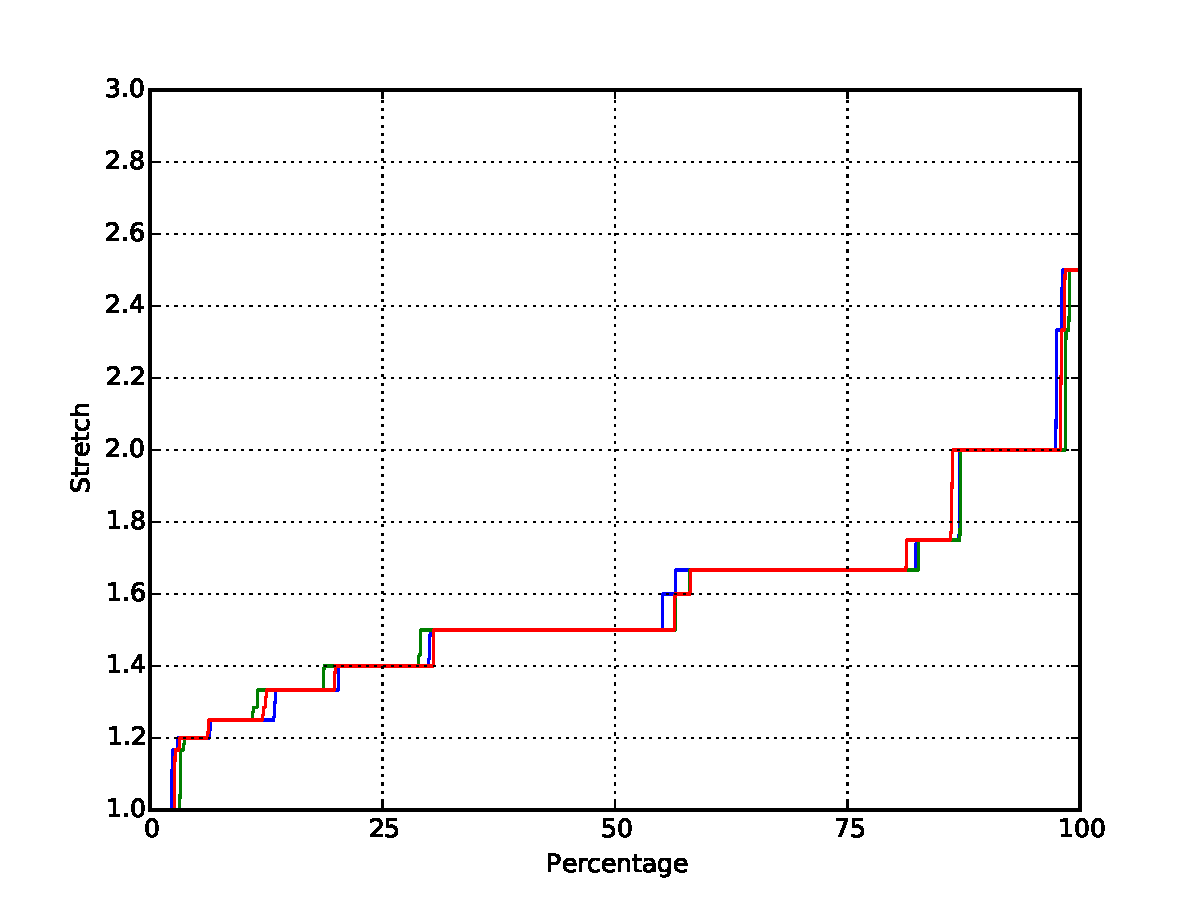
\includegraphics[width=0.8\textwidth]{plots/as_733.pdf}
    \caption{Actual stretches for AS-733 internet topology, the observations
    from each of the three data structures, has been given different colors.}
    \label{fig:as733}
\end{figure}

Again I see similarities between the graphs in this domain.
Even though the graphs differ a lot in size, the average actual stretches is
very close to each other. Also the plots looks very similar, which indicates that
the distribution of the actual stretches is similar for these internet topologies.
\autoref{tab:internettopo} sums up the median, maximum and mean for Skitter
and AS-733.

\begin{table}[htbp]
    \centering
    \begin{tabular}{ l | c | c }
        \toprule
             & Skitter & AS-733 \\
        \midrule
        Median & 1.40 & 1.50 \\
        Max. & 3.0 & 3.0 \\
        \midrule
        Mean. & 1.40 & 1.56 \\
    \end{tabular}
    \caption{Median, maximum and mean for Skitter and AS-733}
    \label{tab:internettopo}
\end{table}
